%!TEX root = ../template.tex
%%%%%%%%%%%%%%%%%%%%%%%%%%%%%%%%%%%%%%%%%%%%%%%%%%%%%%%%%%%%%%%%%%%%
%% chapter2.tex
%% NOVA thesis document file
%%
%% Chapter with the template manual
%%%%%%%%%%%%%%%%%%%%%%%%%%%%%%%%%%%%%%%%%%%%%%%%%%%%%%%%%%%%%%%%%%%%

\typeout{NT FILE chapter2.tex}

\chapter{Related Work}
\label{cha:users_manual}

\glsresetall


\section{Introduction}
\label{sec:introduction}

In this chapter we further detail the issues related to the Centralized Federated Learning Applications and explain why we should use Decentralized Federated Learning Applications as well as how are we expecting to deal with some issues related to delegating helpers to improve systems performance and avoid adverse effects on the functionality of the devices (the network nodes), but first some fundamental subjects will be introduced for a better general understanding of our proposal.


\section{Decentralized Systems}
\label{sec:decentralised_systems}

Decentralized systems are fundamental in distributed computing, enabling tasks to be executed without a central authority.This architectural approach enhances scalability, fault tolerance, and resilience by distributing responsibilities across multiple nodes, allowing them to function autonomously while maintaining coordination. Such systems are particularly valuable in environments that require adaptive and robust communication between a multitude of participants, including \gls{P2P} networks, blockchain technologies, and decentralized applications.\\

In decentralized systems, nodes can dynamically join, leave, or fail without significantly disrupting overall functionality.This is made possible by the use of adaptive protocols that ensure that the system remains operational. Data sharing, connectivity maintenance, and task distribution are facilitated by the deployment of algorithms and protocols. For example, membership protocols guarantee that nodes are aware of each other's presence, whereas peer-to-peer communication models facilitate direct interaction between nodes. Membership protocols serve to ensure that nodes are aware of each other's presence, while \gls{P2P} communication models facilitate direct interaction between nodes.\\

Decentralized systems are a foundational element of modern technologies, including blockchain and decentralized \gls{P2P} file-sharing platforms. These systems demonstrate the potential of decentralization to address scalability and reliability challenges in diverse domains.

\subsection{Membership Protocols}
\label{sub:membership_protocols}

Membership protocols are vital for keeping decentralized swarm systems organized. These systems rely on many individual nodes that interact to accomplish tasks, and each node needs to know which other nodes are active at any moment. 

\begin{enumerate}
  \item \textbf{Epidemic and Scalable Global Membership Service:}
  
  The Epidemic Membership Service works much like spreading a rumor: each node shares information about its presence with a few nearby nodes. These nodes then pass along the update, which eventually reaches the whole network. This approach enables each node to keep a “partial view” of the network, meaning it stays updated on some nodes but not all. This setup keeps the system scalable and ready to handle changes in swarm size. Since updates move organically throughout the network, nodes can join or leave without burdening any single part of the system.
  
  
  \item \textbf{Decentralized Membership Protocols:}
  
  In larger swarms, keeping track of every single node isn’t practical. Decentralized Membership Protocols simplify this by letting each node manage enough information to stay connected without needing to know all nodes. For example, the HyParView protocol organizes nodes into two lists: an active view, which contains frequently updated links to a few critical nodes, and a passive view, a backup list of other nodes. The active view keeps each node actively connected, while the passive view acts as a fallback in case of node failure. This two-layered approach makes HyParView resilient and allows quick recovery if nodes unexpectedly drop out. The protocol is often used within frameworks like Babel, which supports secure and automatic connections. 
     

\end{enumerate}

\subsection{P2P communication}
\label{sec:p2p_communication}

Peer-to-peer (P2P) communication is a decentralized network model in which each peer or node has equal capabilities and responsibilities. \gls{P2P} enables direct communication between nodes, without needing a central authority to mediate the interaction.
  Nodes can connect and disconnect dynamically leading to an architecture that adapts as nodes join or leave the network. 
  These types of networks can scale up or down based on the number of peers. Increasing the number of nodes improves the network's capacity and resilience and decreasing them has limited impact, assuming enough nodes remain active to support data flow. Each node can offer resources, such as processing power or storage capacity, contributing to the overall capacity of the network, this makes \gls{P2P} an efficient approach for apps requiring vast amounts of shared data.
  
  
\begin{figure}[H]
  \centering
  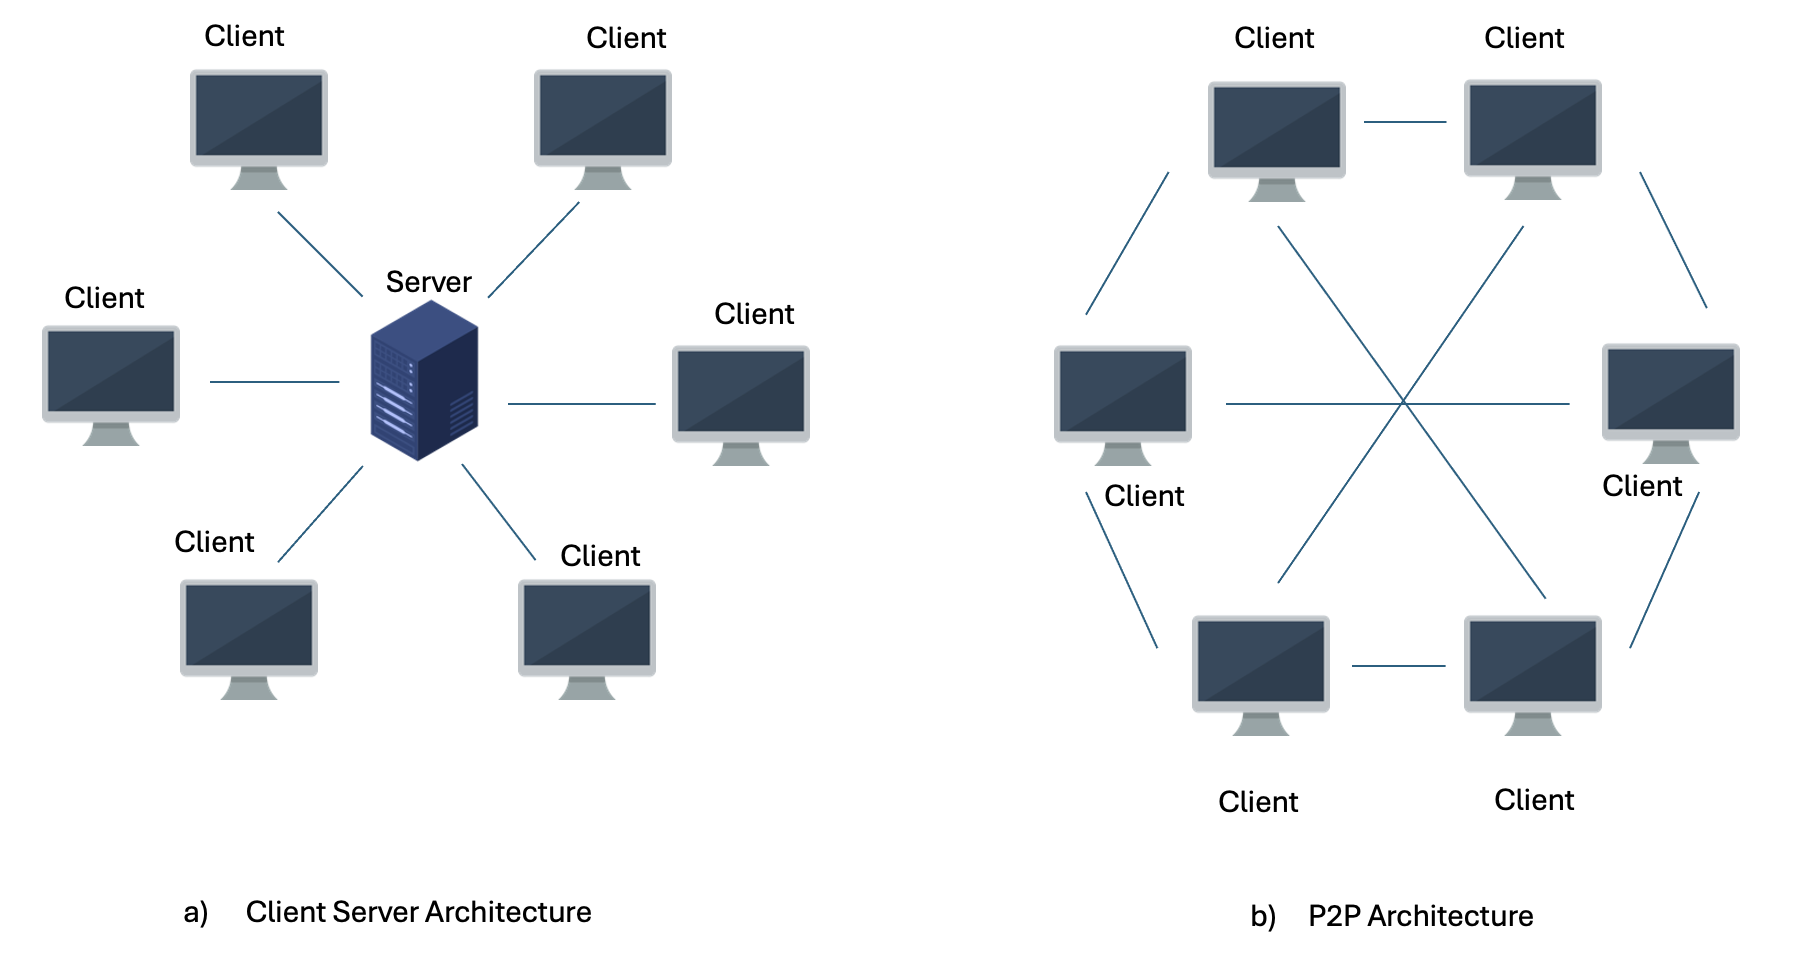
\includegraphics[height=2in]{client-server-vs-p2p}
  \caption{Illustration of client-server and P2P architectures}
  \label{fig:client-server-vs-p2p}
\end{figure}
  
\subsubsection{Broadcast}
\label{sec:Broadcast}

The term broadcast refers to sending messages or data to all peers within a network, since \gls{P2P} networks lack a centralized server, broadcasting relies on each node to propagate the message to others.
This method allows information to spread across the network efficiently, but it also presents challenges related to network congestion, duplication, and ensuring all peers receive the broadcasted message.

Broadcasting can be implemented using various techniques:

\begin{enumerate}

  \item \textbf{Flooding:} In flooding, a peer sends the message to all its directly connected peers, who then forward it to their connected peers, and so on, until the message reaches every peer in the network. This method can lead to message duplication and network congestion, as each peer may receive multiple copies of the same message.
  \item \textbf{Gossip Protocols:} Each node randomly selects a few nodes to send the message, and those nodes, select randomly another subset of their connections, and so on. This method ensures that most or all nodes receive the message without overloading the network.
  \item \textbf{Multicasting:} In structured \gls{P2P} networks, multicasting can be more efficient than broadcasting. Instead of randomly sending messages to every node, it sends only to a specific group/subset of nodes who are most relevant to receive it. This is done by organizing nodes into groups or clusters and sending messages within those or between them.

\end{enumerate}


% subsection with_a_local_latex_installation (end)

\subsection{Decentralized development Frameworks}
\label{sub:decentralized_development_frameworks}

... 

\subsection{Babel}
\label{sub:babel}

Babel is a framework that promotes event driven programming and it helps in the development of distributed protocols within a process that can execute any number of different protocols that communicate with each other, inside or outside the same process. The system is designed with a generic architecture that allows for the implementation of multiple distributed protocols and provides networking components that can capture different capabilities (e.g., \gls{P2P}, Client/Server, ...). 
Babel facilitates the development process by allowing the developer to concentrate on the fundamental aspects of the protocol, without having to address the inherent complications associated with low-level details.

\subsubsection{Babel swarm}
\label{sec:babel_swarm}

....


\section{Federated Learning (FL)}
\label{sec:federated_laerning}

In recent years, Federated Learning (FL) has emerged as a relevant approach for training collaborative models without the need to share sensitive data. Since its emergence, \gls{FL} (\gls{CFL}) has been the predominant methodology in the extant literature, wherein a central entity is responsible for the creation of a global model. However, a centralized approach has the disadvantage of increasing latency due to bottlenecks, heightening vulnerability to system failures, and giving rise to concerns regarding the trustworthiness of the entity responsible for creating the global model. Decentralized Federated Learning (DFL) emerged to address these concerns by promoting decentralized model aggregation and minimizing reliance on centralized architectures.

\begin{figure}[H]
  \centering
  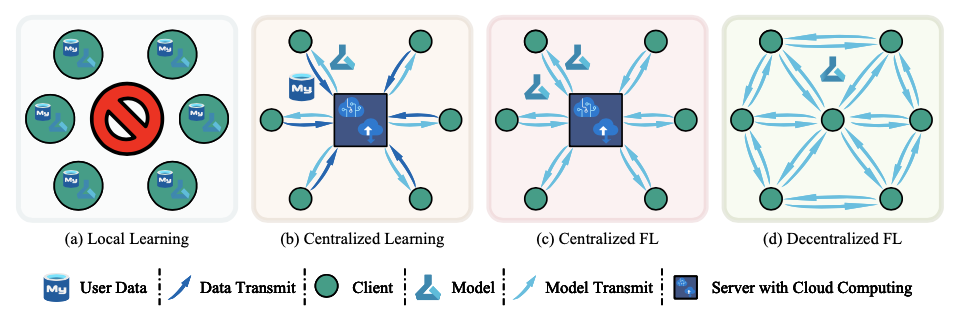
\includegraphics[height=2in]{example_DFL_CFL_DL_LL}
  \caption{Illustration of local learning, centralized learning, CFL, and DFL}
  \label{fig:DFL_CFL_DL_LL}
\end{figure}

Image source: Decentralized Federated Learning: A Survey and Perspective

\subsection{Centralized approach}
\label{sub:fl_centralized_approach}

In \gls{CFL}, a central server is tasked with aggregating updates from local models trained independently on each participant’s data. By exchanging model parameters only and not raw data, this configuration protects data privacy. However, the dependency on a single aggregation server introduces several limitations. Firstly, as the number of participating devices rises, the central server may become a bottleneck, resulting in increased latency and reduced scalability. Additionally, this architecture introduces a potential risk of single-point failure, where the central server’s failure can compromise the integrity of the entire training process. Security and trust are further concerns, as participants must trust the central entity with aggregating and distributing model updates without compromising data privacy.

Due to its simple design and well-established protocols for safe and effective aggregation, \gls{CFL} is still widely used despite all of these disadvantages. In order to minimize the possibility of data leakage, optimization efforts in \gls{CFL} frequently concentrate on lowering communication costs between participants and the server, enhancing the aggregation algorithms, and guaranteeing strong data privacy techniques, such as differential privacy and secure aggregation methods.

\subsection{Decentralized approach}
\label{sub:fl_decentralized_approach}

\gls{DFL} reduces dependency on a central server, which helps to overcome some of the main limitations of CFL. Since model parameters are shared and aggregated in a distributed manner rather than via a single central aggregator, DFL distributes computational responsibility more widely throughout the network.
However, even without a central server, \gls{DFL} still maintains a mechanism for updating a global model through decentralized aggregation strategies, often involving clusters or peer-to-peer structures where nodes collaborate to aggregate model parameters locally before updating the shared model.
This decentralized approach minimizes bottlenecks and reduces the risk of single points of failure, making DFL inherently more fault tolerant and scalable. Additionally, it distributes trust across the entire network rather than concentrating it in a single entity, which can alleviate some concerns about trustworthiness in centralized environments. However, because node interactions are asynchronous, DFL makes it more difficult to maintain consistency in model updates, which can result in stale updates and slower convergence. It also increases communication overhead, as nodes must frequently exchange model parameters with their peers to keep the overall model aligned.
Given that there is no central authority, it can be difficult to detect malicious participants during DFL, making security and privacy issues difficult to resolve. For \gls{DFL} systems to reduce the risk of malicious attacks or data exposure, secure aggregation, anomaly detection, and model update verification require strong, decentralized protocols. These mechanisms are essential to maintain the integrity of the model and the privacy of participants in the decentralized framework. 


\subsection{Discussion}
\label{sub:discussion}

Considering these two approaches, we will focus on Decentralized Federated Learning (\gls{DFL}) to ensure that personal data stays on local devices and is not shared across the network. With \gls{DFL}, only model updates such as parameters and gradients are shared, not the actual data, which helps protect privacy more effectively than a centralized approach.
By choosing \gls{DFL}, our goal is to create a learning network that respects user privacy while remaining resilient and efficient, even as it grows.

\begin{figure}[htbp]
  \centering
  \includegraphics[height=3in]{cfl-vs-dfl}
  \caption{CFL versus DFL}
  \label{fig:dfl_vs_cfl}
\end{figure}

Image source: Decentralized Federated Learning: A Survey and Perspective

\section{Decentralized Federated Learning (DFL)}
\label{sub:decentralized_federated_learning_2}

\gls{DFL} represents an extension of \gls{FL} that eliminates the necessity for a central coordinating server. In contrast, participants communicate directly with one another in a \gls{P2P} network to train a global machine learning model. 

\subsection{\gls{DFL} Architecture}
\label{sub:dfl_architecture}

.......

\subsection{Challenges in federated learning}
\label{sub:challenges_in_fl}

Both CFL and DFL approaches, while innovative in preserving data privacy during collaborative learning, face several critical challenges:

\begin{enumerate}
	\item \textbf{Device and data heterogeneity:}
	
	Participating devices in \gls{FL} differ significantly in terms of available memory, network connectivity, and processing power. Additionally, data from different devices is frequently non-IID (not independently and identically distributed), meaning that each device's data may exhibit distinct patterns. TAs local data from each node can differ from the population as a whole, this lack of uniformity makes it more difficult to create an accurate global model. In \gls{DFL}, the added challenge of device diversity requires adaptive methods for synchronising and aggregating model updates. ​
	\item \textbf{Security and privacy:}
	
	Although FL naturally encourages data privacy by storing data locally, it is still susceptible to a number of attacks because client’s shared parameters and gradients may unintentionally reveal sensitive information. Techniques like model inversion (machine learning security threat that involves using the output of a model to infer some of its parameters or architecture) or membership inference attacks (allows an adversary to query a trained machine learning model to predict whether or not a particular example was contained in the model's training dataset) can exploit these shared updates to reconstruct aspects of the original data or identify if specific data points were involved in training. These vulnerabilities demonstrate the necessity of strong privacy-preserving techniques, like secure aggregation or differential privacy, to reduce data leakage and preserve model performance.
	\item \textbf{Scalability and fault tolerance:} 
	
	While DFL enhances fault tolerance by eliminating single points of failure, scaling DFL networks remains challenging. As the network expands, the demands for communication and synchronisation among nodes grow, which can strain system performance. To manage large numbers of participants efficiently, strategies like effective node clustering, load balancing, and advanced fault tolerance techniques become essential. These methods help distribute workloads more equally across the network and prevent communication bottlenecks, ensuring that model accuracy and system efficiency are maintained as the network scales

\end{enumerate}

\subsection{\gls{ML} Models}
\label{sub:ml_models}

.......

\subsection{Real world Applications}
\label{sub:real_worl_applications}

DFL framework development depends on various key factors, such as relevant application scenarios, sources of information acquisition, information processing units and perceptual prediction modules, among others. And so DFL has been adopted in several areas, such as, automotive industry, healthcare, IoT industry, social networks, etc.

\begin{enumerate}
	\item \textbf{Connected and Automated Vehicles:}
	
	Connected and Automated Vehicles (CAVs) serve as a robust hardware infrastructure for DFL, where each node uses integrated batteries, various sensors, computing units, storage devices and much more. Vehicle-to-vehicle (V2V) communication is a framework that already supports several applications in networks of independent and connected vehicles, creating a basis for the application of Distributed Federated Learning (DFL) in Connected Autonomous Vehicles (CAVs). A V2V approach with FL allows vehicles to share updated knowledge with each other, which is crucial for the safe and efficient operation of vehicle networks. Studies such as that by Lu et al. demonstrate a practical application using Roadside Units (RSUs) act as intermediaries for routing vehicle identities and essential data, facilitating the direct exchange of information between vehicles when necessary. This system, in addition to protecting data privacy, helps reduce the risk of leaking information in vehicular cyber-physical environments (VCPS), enabling safe and efficient collaboration in real time.
	\item \textbf{Mobile Services:}
	
	Mobile services based on IoT devices are an important application scenario for \gls{DFL}, making use of the capabilities of smartphones, PCs, among others. These devices are equipped with several types of sensors and cameras that allow them to collect a big range of information sources. Unlike the relatively fixed connectivity of CAVs, mobile IoT devices offer more flexible systems and platforms to support a wide range of applications.
	\item \textbf{HealthCare:}
	
	Hospital centers and clinics are beginning to shift from \gls{CFL} to \gls{DFL} due to their diverse private data and computing resources. Warnat-Herresthal et al. presented the Swarm Learning, a \gls{DFL} framework that deals with 4 heterogeneous disease use cases, including COVID-19, tuberculosis, leukaemia and lung pathology. The framework incorporates blockchain smart contracts to provide additional security, and dynamically selects leaders to aggregate model parameters at each iteration.
	\item \textbf{Satellites and Unmanned Aerial Vehicles:}
	
	UAVs and satellites in dynamic computing environments have vast amounts of sensitive data for remote sensing, target recognition, and military-related tasks under constraints of limited resources. This makes them suited to the benefits of DFL. Bandwidth is a valuable resource for mobile UAVs and satellites. A potential solution is that the application of a \gls{DFL} framework based on broadcast gossip, customised to dynamic geographical locations, can significantly reduce bandwidth requirements and the consumption of communication resources. Additionally, due to its dynamic nature and highly variable data, \gls{DFL} can also improve real-time responsiveness, adaptability and efficiency of task execution.

\end{enumerate}


\section{Split Learning}
\label{sec:split_learning}

Split learning (SL) has been proposed as a method for enabling resource-constrained devices to train multi-parameter neural networks (NNs) and participate in \gls{FL}. In essence, \gls{SL} divides the \gls{NN} model into sections, enabling clients (devices) to transfer the largest section as a processing task to a computationally robust helper. In SL, it is possible to have multiple helpers that can process model parts of one or more clients, resulting in a notable reduction in the maximum training time across all clients.

In the field of collaborative machine learning, \gls{SL} provides distinct advantages over traditional \gls{FL} by addressing the resource constraints and privacy challenges of small devices such as IoT sensors and mobile devices. SL allows these devices to participate in training complex models by transferring only a portion of the model to powerful helpers, which perform the more computationally intensive tasks. This model split reduces both the memory footprint and computational demand on client devices, which is essential for integrating learning frameworks in environments with limited resources.

\subsection{Advantages of Split Learning}
\label{sec:advantages_of_sl}

SL’s architecture inherently supports several key benefits

\begin{enumerate}
	\item \textbf{Resource Efficiency:} 
	
	By offloading the heaviest computations to a helper, \gls{SL} allows smaller devices to contribute to model training without exhausting their limited resources. This makes SL appropriate for IoT environments and low-processing-power smart devices.
	
	\item \textbf{Device Heterogeneity:} 
	
	SL’s split structure allows it to work across various hardware configurations and network capabilities. For example, SL´s heterogeneous structure enables the workload related to model training to be distributed among devices, helpers, and cloud, taking advantage of diverse computational resources to support scalable networks.
\end{enumerate}

\subsection{SL Architecture}
\label{sec:sl_architecture}

In \gls{SL}, the neural network model is divided into sections, typically at two points called "cut layers". The client device handles the initial layers, which process the raw data. Then, only the activations (or "smashed data") from this initial processing are sent to the server, which takes over the heavier parts of the computation. This division reduces the memory and computational load on the client side and keeps sensitive raw data local, increasing privacy.


\begin{figure}[H]
  \centering
  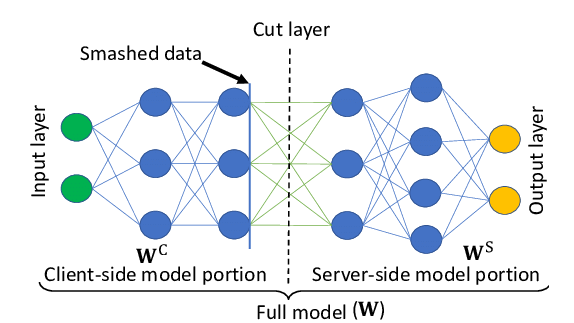
\includegraphics[height=2in]{split-learning}
  \caption{Illustration of split learning architecture}
  \label{fig:DFL_CFL_DL_LL}
\end{figure}


Image source: Advancements of federated learning towards privacy preservation: from federated learning to split learning

\subsection{Applications of Split Learning in Emerging Fields}
\label{sec:application_of_sl_in_emerging_fields}


SL's privacy and resource-efficiency features make it suitable for various domains, including:

\begin{enumerate}
	\item \textbf{Healthcare:}
	
	In collaborative medical AI, hospitals can share insights from their data without sharing actual data. For instance, in diagnosing conditions from imaging data, only processed features are sent to the helper, allowing each hospital to maintain patient confidentiality. \gls{SL} enhance this capability by accelerating training across numerous institutions without centralizing data. Currently, image processing applications in hospital imaging services use this type of mechanism and are already able to detect anomalies and, for example, monitor the development of nodules, comparing old images with current ones. 
	\item \textbf{Smart Cities and 6G Networks:}
	
	SL fits well with the distributed and resource-intensive requirements of future smart cities. SL can support real-time applications such as traffic monitoring and public safety by distributing the computational load across edge servers and mobile devices. In these dynamic configurations, \gls{SL}’s ability to utilize multiple edge nodes in a distributed manner is particularly advantageous. 
	\item \textbf{Autonomous Systems:}
	 
	Autonomous vehicles and drones require frequent updates to machine learning models for tasks like object detection. \gls{SL} enables these devices to offload intensive computations to nearby servers, facilitating real-time updates without overloading on-board systems. ​

\end{enumerate}


\section{Delegation protocols (TBD)}
\label{sec:delegation_protocols}


\begin{enumerate}
	\item \textbf{Request Helper:} \\ When a node detects insufficient processing power for training tasks, it sends a helper request to the delegation service.
	\item \textbf{Helper Assignment:} \\ The delegation service identifies an optimal helper from the membership list and initiates the Babel-based communication protocol to connect the original node with the helper.
	\item \textbf{Session Establishment:} \\ Babel's channel abstraction facilitates creating a communication channel, through which the delegating node and the helper node share training layer information.

\end{enumerate}

....


\section{Helper membership management (TBD)}
\label{sec:helper_membership_management}

\begin{enumerate}
	\item \textbf{Telemetry Monitoring:} \\ Each node sends telemetry data periodically to the delegation service, which includes CPU, GPU usage, RAM, and battery status.

	\item \textbf{Candidate Selection: } \\ Nodes with lower CPU/GPU usage, higher RAM available, and better battery status are prioritized as potential helpers.
	
	\item \textbf{Membership Protocol Adaptation:} \\ Using a gossip or HyParView, can help in maintaining an updated list of potential helper nodes. Babel can support this through its event-driven, message-passing structure for efficient data dissemination​


\end{enumerate}

....

\section{Improvements on Split Learning}
\label{sec:improvements_on_sl}

\gls{SL} as already mentioned is a collaborative machine learning approach that partitions a model between clients and a central server, enabling joint training without sharing raw data. This method offers advantages in privacy preservation and resource efficiency. However, it also presents certain challenges and limitations.
	\\
	Recent advances aim to improve \gls{SL} by addressing the inherent limitations of the approach.

\begin{enumerate}

	\item \textbf{Multi-Level Split Federated Learning (\gls{SFL}):} 
	
	This approach combines the benefits of \gls{SL} and \gls{FL} to improve scalability and reduce communication delays. By introducing a multi-level aggregation architecture, it addresses system and statistical heterogeneity in large-scale AIoT systems with non-IID data distributions.
	
	\item \textbf{SplitFed Learning without Client-Side Synchronization:}
	 
	Traditional SplitFed Learning requires synchronization among clients, leading to communication and computation overhead. An alternative approach removes this requirement, resulting in a "Multi-head Split Learning" architecture. Empirical studies indicate that this method achieves performance comparable to traditional SplitFed Learning while reducing client-side overhead. 

\end{enumerate}

\subsection{Open Challanges}
\label{sec:sl_open_challenges}

Several studies have identified challenges in SL that remain unresolved, such as Privacy Leakage which despite \gls{SL}'s design to protect data privacy, research has demonstrated the existence of potential vulnerabilities that could allow adversaries to reconstruct the original data from gradients or shared activations. This suggests that \gls{SL} may not provide comprehensive protection for sensitive information.

\subsection{Limitations of Existing Solutions}
\label{sec:limitations_on_existing_solutions}

While enhancements have been proposed, certain limitations remain:

\begin{enumerate}
	\item \textbf{Communication Overhead:}
	
	Some solutions, such as traditional \gls{SFL}, introduce considerable communication overhead due to the necessity for client-side synchronization. This can prove to be a significant burden for devices with limited resources. 
	
	\item \textbf{Scalability Issues:}
	
	Despite the fact that multi-level \gls{SFL} is designed to enhance scalability, it may still face challenges in the context of extremely large and heterogeneous networks, particularly when confronted with non-IID data distributions.
	
	These factors described below, once combined, can make efficient scaling difficult in some environments:
	
	\subitem \textbf{Diverse Data Patterns:}
	
	 Non-IID data means each client has significantly different data, making it harder to train a unified model that performs well for everyone.
	 
	 \subitem \textbf{Resource Constraints:}
	 
	 Large networks often involve devices with varying computational power, causing delays and inefficiencies during training.
	 
	 \subitem \textbf{Communication Bottlenecks:}
	 
	 As the network grows, the amount of data exchanged increases, leading to delays and higher costs in synchronizing updates across devices.

\end{enumerate}


\subsection{Discussion}
\label{sec:sl_improvements_discussion}

Our proposed solution addresses the aforementioned limitations by staying with "normal" \gls{SL} rather than adopting \gls{SFL}, due to its significantly simpler development and operational advantages:

\begin{enumerate}
	\item \textbf{Enhances Privacy: }
	
	By keeping the focus on standard Split Learning, our approach reduces the complexity of client-side synchronization, minimizing the risk of additional data leakage through intermediate synchronization steps required in SplitFed Learning.
	
	\item \textbf{Reduces Communication Overhead:}
	
	Split Learning inherently involves fewer data exchanges compared to SplitFed Learning, as it avoids the frequent client-to-client synchronization that \gls{SFL} requires. This results in a more efficient and streamlined communication process.

	\item \textbf{Simplifies Development:} 
	
	The development of SplitFed Learning is notably more complex due to the need to coordinate and synchronize updates across multiple clients. By using SL, our solution maintains a straightforward and more manageable architecture.
	
\end{enumerate}

By focusing on standard \gls{SL}, our solution prioritizes simplicity and efficiency while addressing key challenges in collaborative machine learning, making it a robust and practical choice for real-world applications.



\section{FL apps/frameworks used to train models and classify sets}
\label{sec:fl_apps_and_frameworks}

Machine learning as a service (MLaaS) has increased in recent decades due to increased collection and processing of big data, availability of public APIs, new advanced machine learning (\gls{ML}) methods, open source libraries, tools for \gls{ML} analysis large-scale and cloud-based computing. These types of systems tended to be predominantly centralized, but with the emergence of Federated Learning due to concerns in terms of privacy, scalability and devices diversity, new services more dedicated to Federated Learning have started to appear, the so called Federated Learning as a Service. Below will be presented some of these services.

\begin{enumerate}
	\item \textbf{TensorFlow Federated (TFF):}
	
	...
	\item \textbf{Flower:}
	 
	...
	\item \textbf{PySyft by OpenMined:}
	 
	...
	\item \textbf{OpenFL by Inte:}
	 
	...
	\item \textbf{FLaaS by Telefónica:}
	
	...
	
\end{enumerate}


\subsection{Discussion}
\label{sec:discussion_fl_apps_frameworks}

....

\section{LaTeX}

\subsection{Class of Text}
\label{sub:class_of_text}

You must choose the class of text for the document. The available options are:

\begin{enumerate}
  \item \textbf{bsc} --- BSc graduation report.
  \item \textbf{*mscplan} --- Preparation of MSc dissertation. This is a preliminary report graduate students at DI-FCT-NOVA must prepare to conclude the first semester of the two-semesters MSc work. The files specified by \verb!\ntdedicatoryfile! and \verb!\acknowledgmentsfile! are ignored, even if present, for this class of document.
  \item \textbf{msc} --- MSc dissertation.
  \item \textbf{phdprop} ---  Proposal for a PhD work. The files specified by \verb!\ntdedicatoryfile! and \verb!\acknowledgmentsfile! are ignored, even if present, for this class of document.
  \item \textbf{prepphd} ---  Preparation of a PhD thesis. This is a preliminary report PhD students at DI-FCT-NOVA must prepare before the end of the third semester of PhD work. The files specified by \verb!\ntdedicatoryfile! and \verb!\acknowledgmentsfile! are ignored, even if present, for this class of document.
  \item \textbf{phd} --- PhD dissertation.
\end{enumerate}
% subsection class_of_text (end)

% ============
% = Printing =
% ============
\subsection{Printing}
\label{sub:printing}

You must choose how your document will be printed. The available options are:
\begin{enumerate}
  \item \textbf{oneside} --- Single side page printing.
  \item \textbf{*twoside} --- Double sided page printing.
\end{enumerate}
% subsection printing (end)

% =============
% = Font Size =
% =============
\subsection{Font Size}
\label{ssec:font_size}

You must select the encoding for your text. The available options are:
\begin{enumerate}
  \item \textbf{11pt} --- Eleven (11) points font size.
  \item \textbf{*12pt} --- Twelve (12) points font size. You should really stick to 12pt\ldots
\end{enumerate}
% subsection font_size (end)

% =================
% = Text encoding =
% =================
\subsection{Text Encoding}
\label{ssec:text_encoding}

You must choose the font size for your document. The available options are:
\begin{enumerate}
  \item \textbf{latin1} --- Use Latin-1 (\href{http://en.wikipedia.org/wiki/ISO/IEC_8859-1}{ISO 8859-1}) encoding.  Most probably you should use this option if you use Windows;
  \item \textbf{utf8} --- Use \href{http://en.wikipedia.org/wiki/UTF-8}{UTF8} encoding.    Most probably you should use this option if you are not using Windows.
\end{enumerate}
% subsection font_size (end)

% ============
% = Examples =
% ============
\subsection{Examples}
\label{ssec:examples}

Let's have a look at a couple of examples:

\begin{itemize}
  \item Preparation of PhD thesis, in portuguese, with 11pt size and to be printed single sided (I wonder why one would do this!)\\
  \verb!\documentclass[prepphd,pt,11pt,oneside,latin1]{thesisdifct-nova}!
  \item MSc dissertation, in English, with 12pt size and to be printed double sided\\
  \verb!\documentclass[msc,en,12pt,twoside,utf8]{thesisdifct-nova}!
\end{itemize}
% subsection examples (end)

\section{How to Write Using \LaTeX}
\label{sec:how_to_write_using_latex}

Please have a look at Chapter~\ref{cha:a_short_latex_tutorial_with_examples}, where you may find many examples of \LaTeX constructs, such as Sectioning, inserting Figures and Tables, writing Equations, Theorems and algorithms, exhibit code listings, etc.

% section how_to_write_using_latex (end)




% \printbibliography[heading=subbibliography, segment=\therefsegment, title={\bibname\ for chapter~\thechapter}]

